\chapter{Render Large Lists with SectionList}

\section{Video: Render large lists by sections using SectionList}
\subsection{Why SectionList?}
\begin{itemize}
    \item The entire menu rendered with FlatList is presented as one long uninterrupted list. 
    \item To make things tidy, divide the list into sections.
    \item SectionLists has the same features found in FlatList component, but it also supports the separation of items in the lists.
\end{itemize}

\subsection{Comparision between FlatList and SectionList components}
\begin{itemize}
    \item FlatList and SectionList use the same lazy rendering and inherits the props of the ScrollView.
    \item SectionList support break the layout into smaller chunks and add appropriate child-headers.
    \item \textbf{Practice Question:} Which of the following are characteristics of the \texttt{SectionList} component? Select all that apply.
    $\rightarrow$ It uses lazy rendering, It supports section headers and separators, It inherits props of the \texttt{ScrollView} component.
\end{itemize}

$\rightarrow$ SectionList improves performance and enables to present the menu items in a more pleasant and easy to read.

\subsection{Syntax}
\textbf{SectionList component syntax}
\begin{lstlisting}[language=Java, numbers=none]
    <SectionList
        sections={items} // Array of list sections
        renderItem={renderItem} // Default renderer
    />
\end{lstlisting}
\begin{itemize}
    \item The sections must follow this structure:
    \begin{lstlisting}[language=Java, numbers=none]
        [
            {
                title: '',
                data: []
            },
            ...
        ]
    \end{lstlisting}

    \item Then \texttt{renderItem} uses the below props, which the item is each item of \texttt{data} array.
    \item The \texttt{renderSectionHeader} need to pass the single section, then extract the title from those section.
\end{itemize}

\textbf{renderItem syntax}
\begin{lstlisting}[language=Java, numbers=none]
    renderItem({ item, index, section, separators });

    /*
        item: section data key
        index: item position in section
        section: section object
        separators: contains special functions
    */
\end{lstlisting}

\subsection{Some props could be passed into SectionList}
\begin{itemize}
    \item Header
    \item Footer
    \item Separators
    \item ...
\end{itemize}

\section{Video: Using the SectionList component}
\begin{itemize}
    \item \textbf{Practice Question:} You are creating a ‘Contact’ page for your React Native app that separates contact details into sections such as email, phone, and social media. In your \texttt{SectionList} component, which property would you use to extract the data from the array to render these section headers?  
    $\rightarrow$ renderSectionHeader 

    \item The iOS's Header of each section sticks to the top of the SectionList.
    \item Its not applied for Android.
\end{itemize}

\section{Reading: Explore the SectionList component}
\begin{figure}[H]
    \centering
    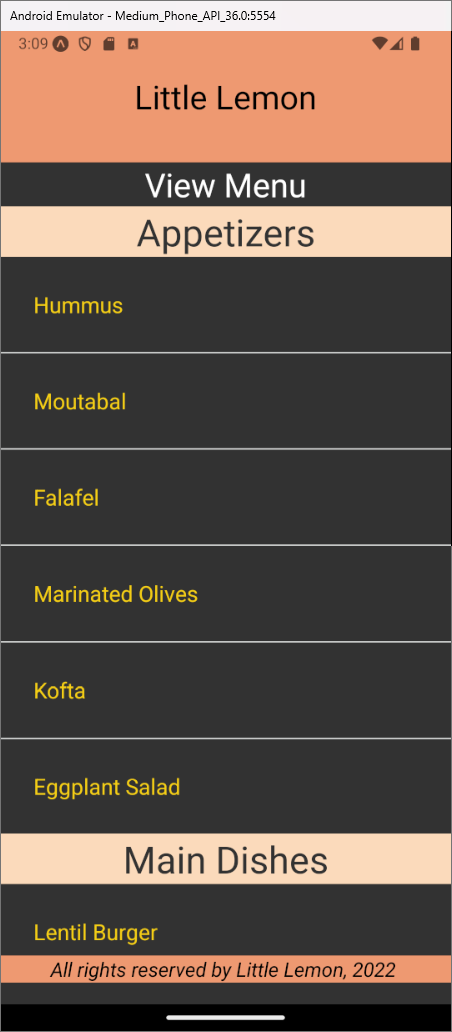
\includegraphics[width=0.2\textwidth]{images/ex2.png}
    \caption{Exercise: Explore the SectionList component}
\end{figure}

\section{Reading: Exercise: Render a large list using SectionList}
\begin{figure}[H]
    \centering
    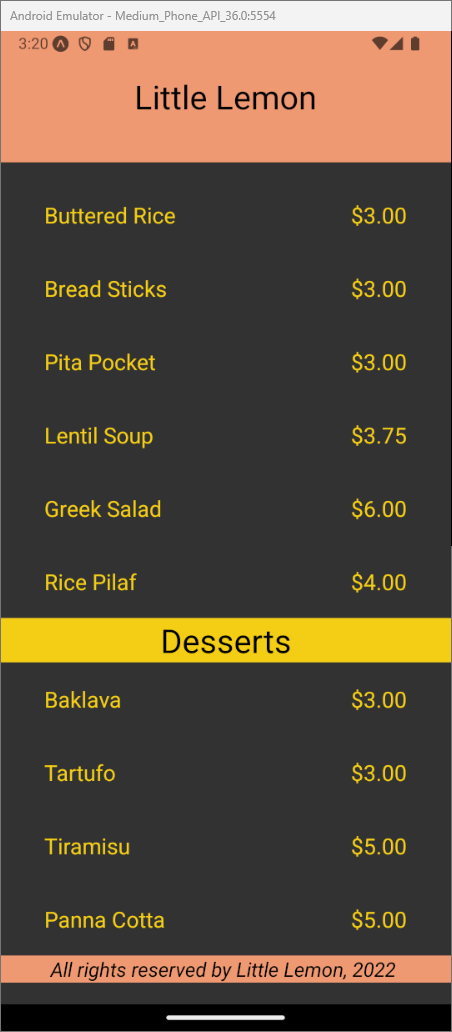
\includegraphics[width=0.2\textwidth]{images/Ex3.png}
    \caption{Exercise: Render a large list using SectionList}
\end{figure}

\section{Practice Assignment: Self review: Render a large list using SectionList}
\begin{figure}[H]
    \centering
    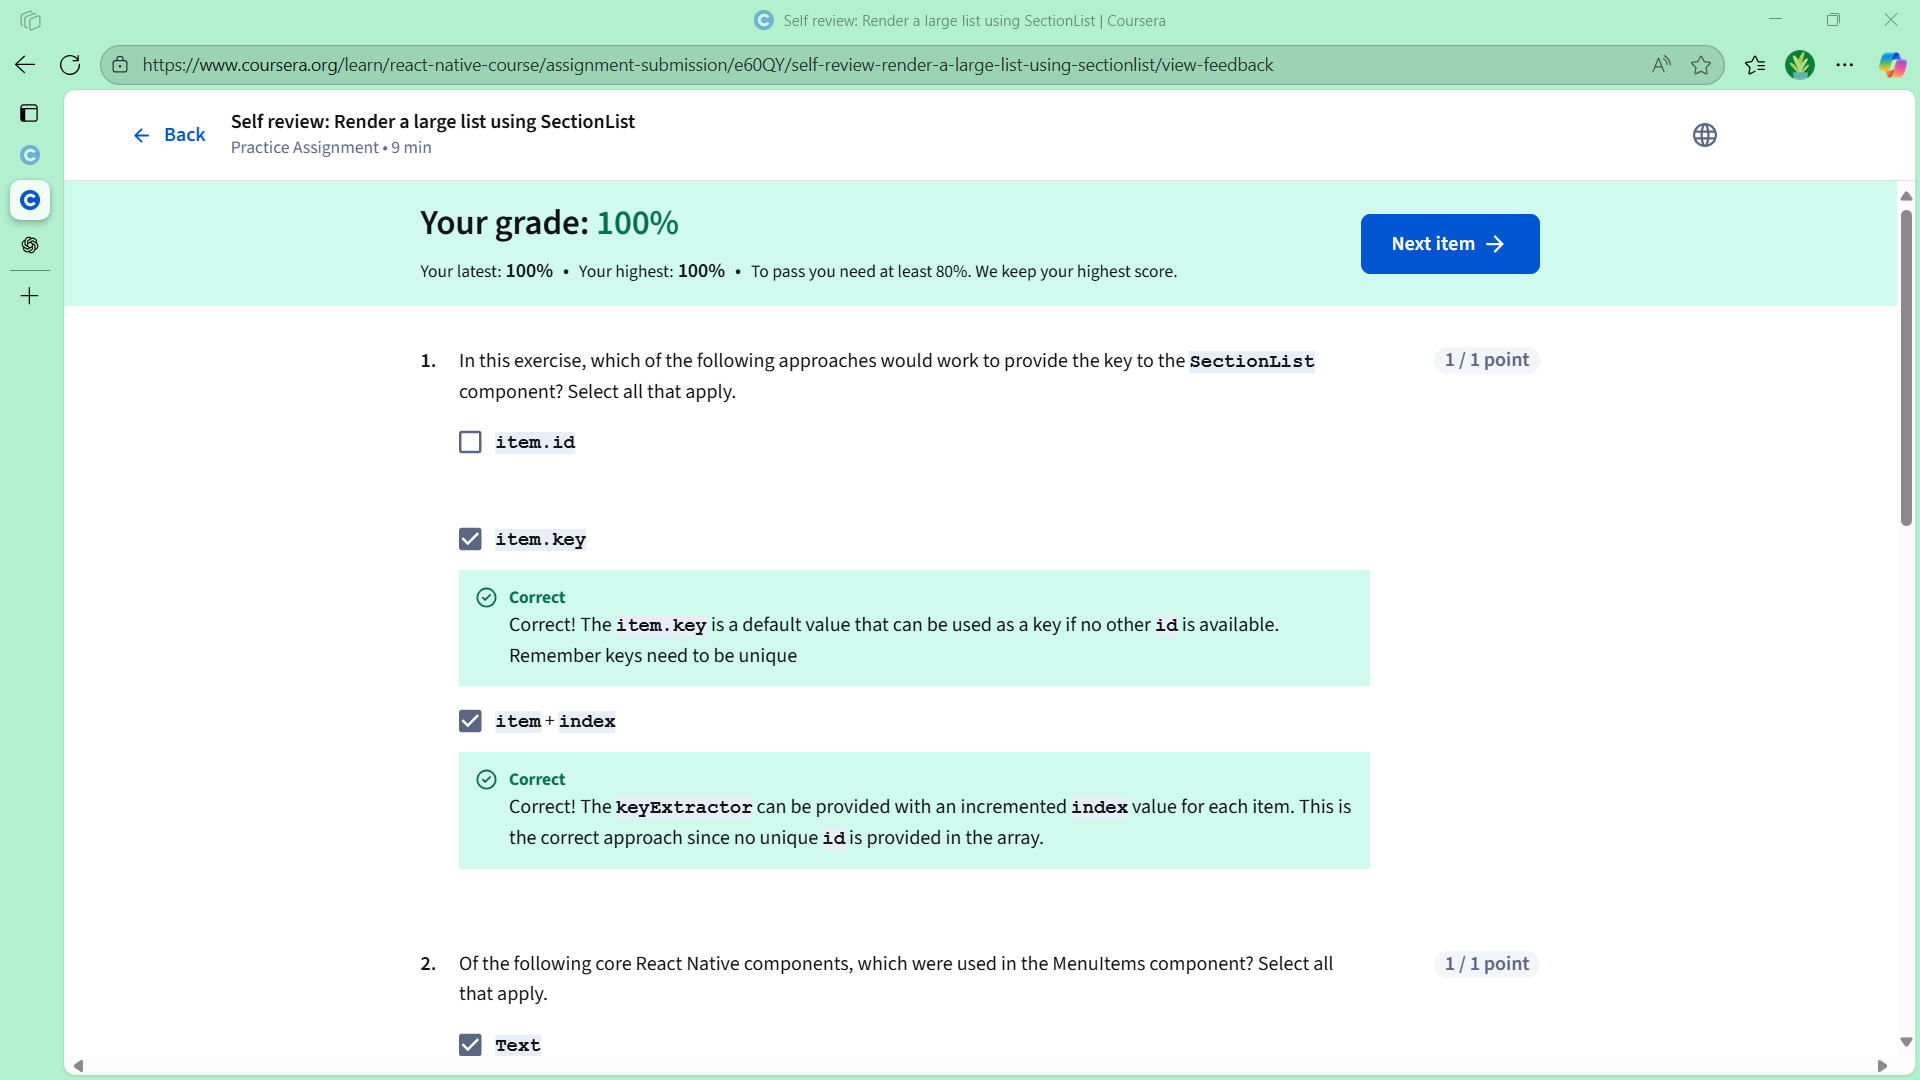
\includegraphics[width=0.5\textwidth]{images/sr-2.png}
    \caption{Self review: Render a large list using SectionList}
\end{figure}

\section{Practice Assignment: Knowledge checking: Render a large list using SectionList}
\begin{figure}[H]
    \centering
    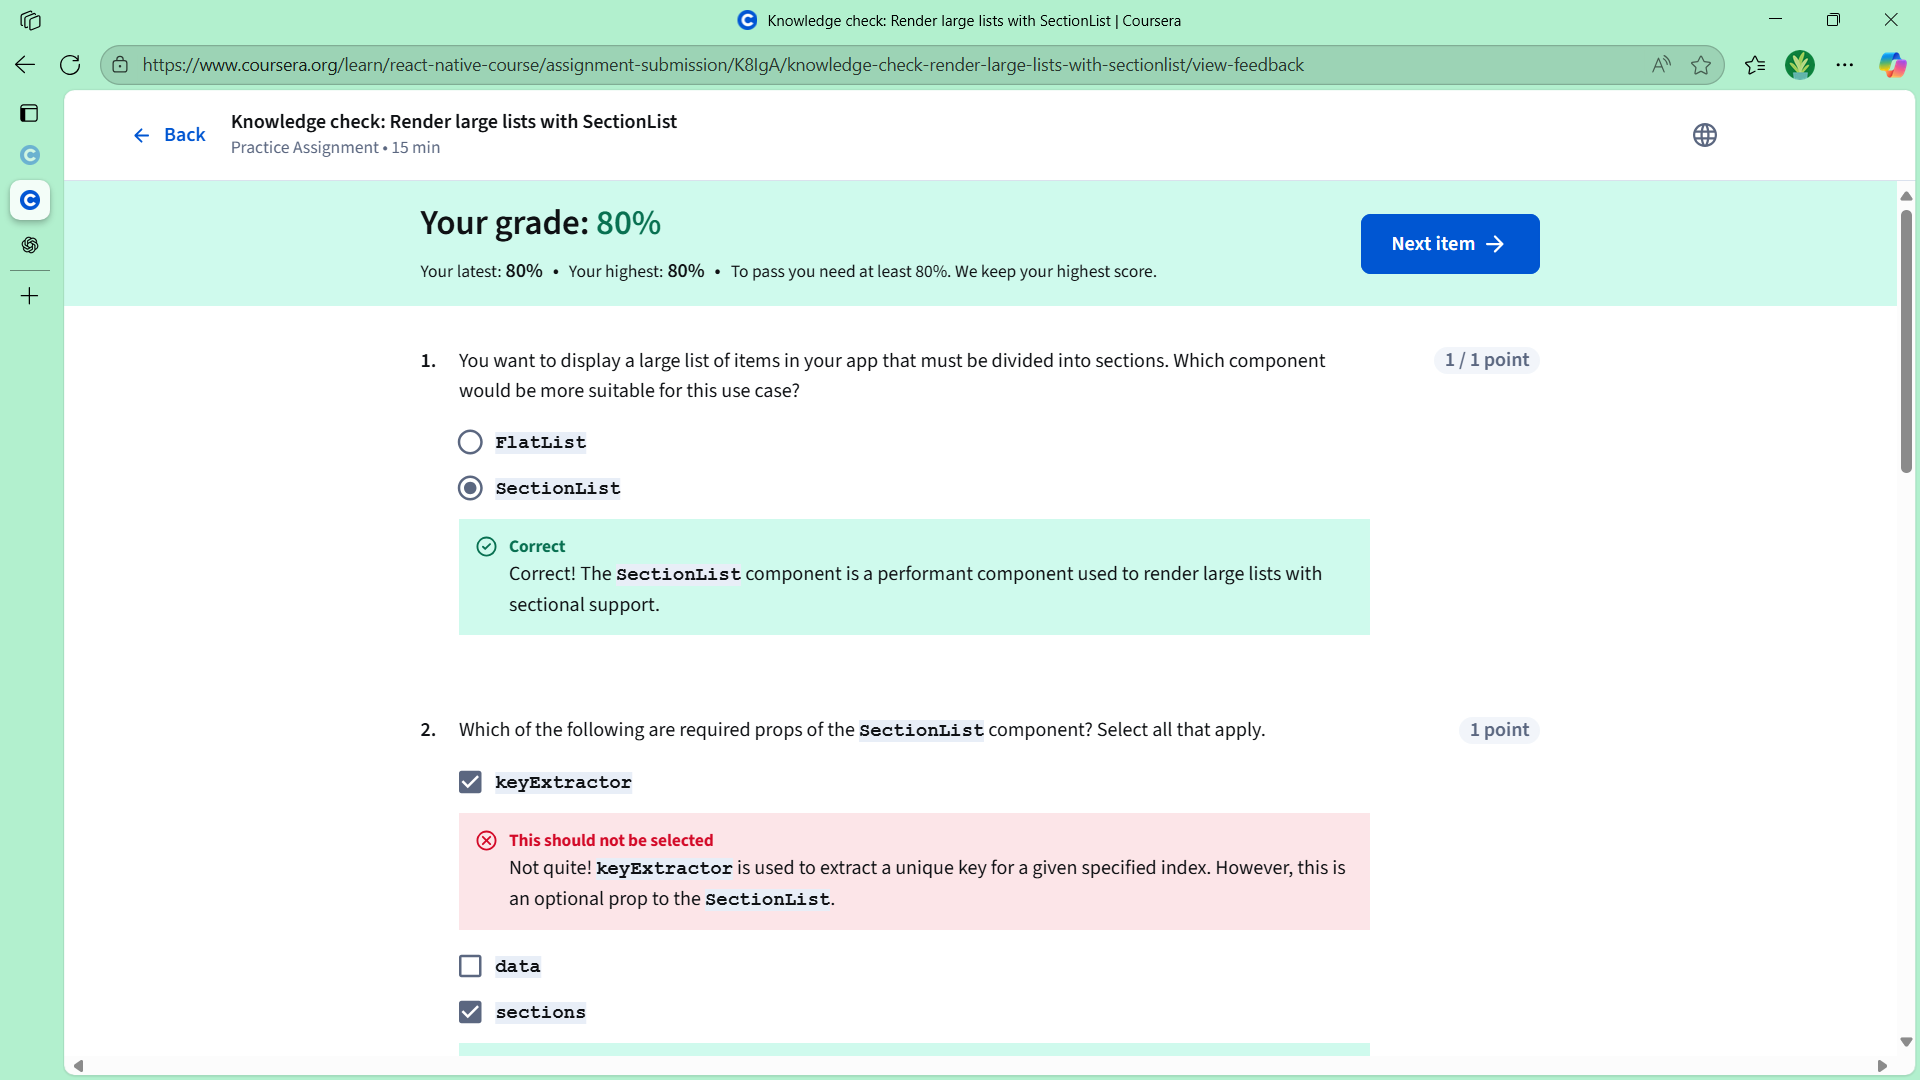
\includegraphics[width=0.5\textwidth]{images/kc-2.png}
    \caption{Knowledge Check: Render a large list using SectionList}
\end{figure}